
\documentclass[11pt,a4paper]{article}

\usepackage[parfill]{parskip}
\usepackage{epsfig}
\usepackage{amsmath}
\usepackage{array, multirow, color, colortbl}
\usepackage{hyperref, longtable}
\hypersetup{
	colorlinks=true,
	linkcolor=blue,
	filecolor=magenta,      
	urlcolor=cyan,
}

\setlength{\parindent}{0pt}
\setlength{\parskip}{5pt}

\setlength{\evensidemargin}{0cm} \setlength{\oddsidemargin}{0cm}
\setlength{\topmargin}{-1cm} \setlength{\textwidth}{16cm}
\setlength{\textheight}{24.5cm}

\pagestyle{plain}

\renewcommand{\baselinestretch}{1.2}
\newcommand{\com}[1]{\textcolor{red}{[#1]}}
\newcommand{\prep}[1]{\textcolor{blue}{#1}}

% Set up a command to produce grey boxes in tables
\newcommand{\grb}{\cellcolor[gray]{0.8}}
\newcommand{\tmmathbf}[1]{\ensuremath{\boldsymbol{#1}}}

%----------------------------------------------------------------------------Definitions
%%%% vectors
\newcommand{\fett}[1]{\boldsymbol{#1}}
\renewcommand{\vec}[1]{\fett{#1}}



%------------------------------------------------------------------------------
\begin{document}

\hrule\vspace{2mm} 
\centerline{\large   ENGINEERING TRIPOS PART IIA}
\vspace{0.5cm} \centerline{ \large \bfseries LOCATION: DPO  \hfill EXPERIMENT 3D7}
\vspace{0.5cm} \centerline{ \large \bfseries FINITE ELEMENT METHOD}
\vspace{2mm}
\hrule
%

%
%------------------------------------------------------------------------------
\section*{Summary} 
%------------------------------------------------------------------------------
%
In this lab exercise the finite element method will be used to analyse the tensioned strip with a circular hole previously considered in the 3C7 lab. 

%
%------------------------------------------------------------------------------
\section*{Objectives} 
%------------------------------------------------------------------------------
%
\begin{itemize}
\item Use a finite element package to solve linear elasticity equations

\item Generate finite element meshes using a mesh generator

\item Identify and define appropriate boundary conditions

\item Compare finite element results with experimental measurements and analytical solutions 

\item Analyse the influence of the mesh refinement on the final results
\end{itemize}

\vspace{0.5 cm} 
\hrule

\paragraph{Important:} Before coming to the lab read this handout and load the Jupyter notebook on Google Colab %
\href{https://colab.research.google.com/github/fcirak/3D7Lab/blob/main/notebook/3D7-lab-notebook-v2.ipynb}{here}. Make sure the notebook it is running (use your university google account). Compare the equations given in this handout and their implementation in the notebook.

%\section{Introduction}

%In this lab you will use the open-source finite-element package \href{https://fenicsproject.org/}{FEniCS} and the mesh generator \href{https://gmsh.info/}{gmsh} to solve the stress field in the vicinity of a circular hole in a plate under uniaxial tension. All instructions for running the software are included in the google colab notebook.

%
%------------------------------------------------------------------------------
\section{Problem description \label{s:problem}}
%------------------------------------------------------------------------------
%
This lab exercise involves performing finite element analyses of a tensioned strip with a circular hole using various meshes. The quantity of interest is the stress field in the strip. The meshes are generated with \href{https://gmsh.info/}{gmsh} and the finite element analysis is performed with \href{https://fenicsproject.org/}{FEniCS}.  All instructions for running both are included in the google colab notebook.  \\

\noindent
The strip has the width $100$~mm, length $300$~mm, thickness $1.7$~mm and  hole radius $R = 14.8$~mm. The Young's modulus is $E = 70$~GPa and Poisson's ratio is $\nu = 0.33$. The strip is subjected to uniform tension of $\sigma_0$ applied at its two ends through. The total applied force is $F=10$ kN. Due to symmetry, it is sufficient to model one quarter of the strip as shown in Figure~\ref{fig-geometry}. 


\begin{figure}[htb]
    \centering
     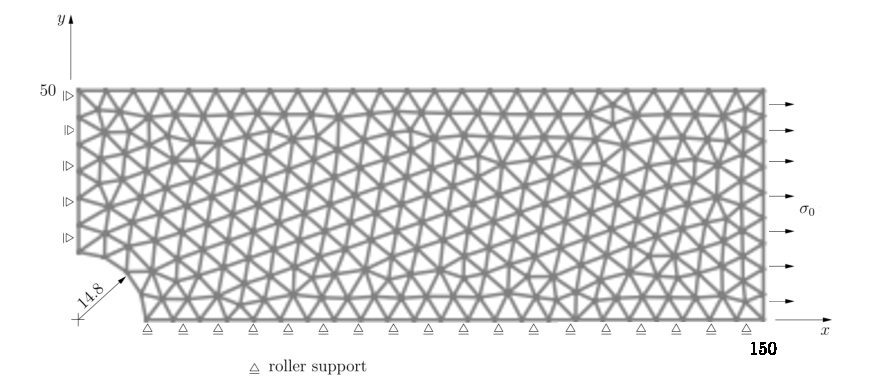
\includegraphics[width=400pt]{figs/dessin.pdf}	
    \caption{Geometry of one quarter of the strip.}
    \label{fig-geometry}
\end{figure}

%
%------------------------------------------------------------------------------
\section{Finite element model \label{s:model}}
%------------------------------------------------------------------------------
%
%The first step in the analysis is to define the finite element model. To that end, we start by deriving the equations of elasticity in weak form. We then determine appropriate boundary conditions and define the mesh and the element type for our analysis.

%
%------------------------------------------------------------------------------
\subsection{Equilibrium equations in strong and weak form}
%------------------------------------------------------------------------------
%
In planar elasticity the primary unknown is the displacement field with two components 
%
\begin{equation}
	\vec u = 
	\begin{bmatrix}
	u_x \\
	u_y
	\end{bmatrix}
\end{equation}
%
%
The axial strains~$\epsilon_{xx} $ and $\epsilon_{yy}$,  and the shear strain~$\epsilon_{xy}$  are given by
%
\begin{align}
\begin{split}
	\epsilon_{xx} &= \frac{\partial u_x}{\partial x}  \\
	\epsilon_{yy} &= \frac{\partial u_y}{\partial y} \\
	\epsilon_{xy} &= \frac{1}{2} \gamma_{xy} =  \frac{1}{2} \left (\frac{ \partial u_y}{\partial x} + \frac{\partial u_x}{\partial y} \right ) \, .
\end{split}	
\end{align}
%
Notice that this definition implies $\epsilon_{xy}=\epsilon_{yx}$. In computer implementations of the finite element method, it is convenient to  arrange the strains in a column vector 
%
\begin{equation}
\vec \epsilon = 
\begin{bmatrix}
\epsilon_{xx} \\
\epsilon_{yy} \\
2\epsilon_{xy}
\end{bmatrix}
= 
\begin{bmatrix}
\frac{\partial }{\partial x} & 0 \\[0.3em]  
0 & \frac{\partial }{\partial y} \\[0.3em] 
\frac{\partial }{\partial y} & \frac{\partial }{\partial x}
\end{bmatrix}
\begin{bmatrix}
u_x \\
u_y
\end{bmatrix}
\end{equation}
%
This equation is written in a more compact form using the {\em symmetric gradient operator} $\vec\nabla_S $, that is,
%
\begin{equation}
\vec \epsilon = \vec \nabla_S \vec u  \quad \text{with} \quad \vec \nabla_S =
\begin{bmatrix}
\frac{\partial }{\partial x} & 0 \\[0.3em]  
0 & \frac{\partial }{\partial y} \\[0.3em]  
\frac{\partial }{\partial y} & \frac{\partial }{\partial x}
\end{bmatrix}
\end{equation}
%

The equilibrium equations in component form are given by 
%
\begin{align}
\begin{split}
\frac{\partial \sigma_{xx}}{\partial x} + \frac{\partial \sigma_{xy}}{\partial y}  & = 0 \\
\frac{\partial \sigma_{yx}}{\partial x} + \frac{\partial \sigma_{yy}}{\partial y} &=0
\end{split}
\end{align}
%
Notice that there are no distributed body forces in this example.  The equilibrium equations can be written as 
%
\begin{equation}
\begin{bmatrix}
\frac{\partial }{\partial x}  & 0 & \frac{\partial }{\partial y} \\[0.3em] 
0 & \frac{\partial }{\partial y} & \frac{\partial }{\partial x}
\end{bmatrix}
\begin{bmatrix}
\sigma_{xx}  \\ \sigma_{yy} \\ \sigma_{xy}
\end{bmatrix}
= 
\begin{bmatrix}
0 \\ 0 
\end{bmatrix} \, , 
\end{equation} 
%
or more compactly as 
%
%
\begin{equation}
 \vec \nabla_S^T \fett \sigma  = \vec 0 \, .
\end{equation}
%
%


The strains~$\vec \varepsilon$ and stresses~$\vec \sigma$ are related to each other through  Hooke's law.  The generalisation of Hooke's law to two dimensions can be written as
%
\begin{equation}
	\vec \sigma = \vec D \vec \varepsilon \, .
\end{equation}
%
The matrix~$\vec D$ depends on whether plane stress or plain strain conditions are assumed. A plane stress model is appropriate because the considered strip is relatively thin so that the through-thickness stress is zero. According to the Data Sheet, the~$\vec D$ matrix for plane stress is 
%
\begin{equation}
\vec D = \frac{E}{1-\nu^2} 
\begin{bmatrix}
1 & \nu & 0 \\
\nu & 1 & 0 \\
0 & 0 & (1-\nu)/2
\end{bmatrix} \, .
\end{equation} 
% 

The weak form of the elasticity equations is the principle of virtual work which you already know from Part I of your studies. As it will be derived in the lectures the weak form is given by 
%
\begin{equation} \label{eq:weakform}
\int_\Omega (\vec \nabla_S \vec w)^T \fett \sigma (\vec u) \, d\Omega = \int_{\Gamma_t} \vec w^T \overline{\fett t} \, d \Gamma_t  \, , 
\end{equation}
%
where~$\vec w$ is the \underline{test function}, $\vec u$ is the \underline{trial function}, and~$\overline{\vec t} = \begin{bmatrix}  \overline t_x & \overline t_y \end{bmatrix}^T$ is the applied traction on the \underline{Neumann boundary}~$\Gamma_t$.



%
%------------------------------------------------------------------------------
\subsection{Boundary conditions}
%------------------------------------------------------------------------------
%
\paragraph{Essential (Dirichlet) boundary conditions} The displacement of all nodes on the symmetry line must be constrained to be zero in the direction normal to the line. At the same time, these nodes should be free to move parallel to the line. 

The finite element model must have sufficient constraints to prevent rigid body motion. If rigid body motion is possible  the stiffness matrix will be singular, or rank deficient.   


\paragraph{Natural (Neumann) boundary conditions}

The natural boundary condition appears in the right-hand side of the weak form~\eqref{eq:weakform}. The value of the traction~$\overline{t}_x$ is found by dividing the total applied force ($F = 10 \, kN$) by the cross-sectional area ($100 \, mm \times 1.7 \, mm$) \mbox{$\Rightarrow \sigma_0 \approx  58.8\,  N/mm^2$}. 
%
%------------------------------------------------------------------------------
\subsection{Influence of the mesh and element type}
%------------------------------------------------------------------------------
%

You will define several meshes as described below, using triangular elements. You should always make sure that the element aspect ratio (i.e., length/width) is less than three and never greater than five in order to limit numerical errors due to an ill-conditioned stiffness matrix. When defining graded meshes, use small elements in regions of large stress gradient or where high accuracy is required.
%
\begin{itemize}
\item A uniform mesh of approximately 250 triangular elements. %This mesh should have approximately 300 degrees of freedom if the elements are linear.
\item A uniform mesh of approximately 15000 triangular elements.
%This mesh should have approximately 60000 degrees of freedom if the elements are quadratic.
\item A mesh with approximately 250 triangular elements. 
%This mesh should have approximately 1100 degrees of freedom if the elements are quadratic. 
Adjust the number of elements and their size distribution to create a graded mesh in-line with the advice given above. The objective is to obtain the greatest accuracy with the limited number elements. This will be by trial and error.
\end{itemize}
%


%
%------------------------------------------------------------------------------
\section{Off-centre hole analysis.}
%------------------------------------------------------------------------------
%

\textit{This section is optional for the standard laboratory. In the Laboratory Report, results
from this analysis are not required. Students using this laboratory exercise for their Full
Technical Report must do this analysis in full and discuss it in their report. A script for the generation of a mesh corresponding to this new geometry can be copied from \href{https://colab.research.google.com/github/fcirak/3D7Lab/blob/main/notebook/3D7-mesh-FTR-v0.ipynb}{here} and used in the jupyter notebook.}

Using a very fine reference mesh with linear triangles and a mesh of quadratic triangles
with no more than 600 degrees of freedom, analyse the same plate (length, width and thickness are identical to the previous section) with
an off-centre hole. The plate is subjected to uniform tension of $\sigma_0$ applied at its two ends through a tensometer. The total applied force is $F=10$ kN. The distance
of the hole centre from the centre-line is $e = 16$ mm and the radius of the hole again
is $R = 14.8$ mm. The material properties are the same as those used above. Begin
by making a sketch of the boundary value problem to analyse (taking into account any
symmetries) and then adjust the number of elements and their size distribution in-line
with the advice given in section~\ref{s:problem} to obtain the greatest accuracy with these limited
number of nodes. Plot the distributions of horizontal and vertical stress along axes passing through the
centre of the hole and parallel to the sides of the plate.

%
%------------------------------------------------------------------------------
\section{Write-ups}
%------------------------------------------------------------------------------
%
You should refer to the advice given in the General Instructions document Sections 2.2
and 2.3.
%
%------------------------------------------------------------------------------
\subsection{The Laboratory Report [3 hours]}
%------------------------------------------------------------------------------
%
\textit{This report should be submitted online within 15 days of your second lab session, latest at 4pm.}  \\


This should be word-processed and no more than three pages, excluding any diagrams
and graphs. The report pertains only to the centred hole problem of section~\ref{s:problem} and should
contain the following in addition to any other issues that you may wish to discuss.
%
\begin{itemize}
\item Along the horizontal and vertical axes, plot the vertical and horizontal stress distributions calculated with the different meshes. Compare these stresses with those obtained for a hole in an infinite
plate that is stretched uniformly and also compare the stress at the periphery of
the hole with Howland's analytical solution, see Appendix B.
\item On the same graph plot the stresses measured experimentally (you can download these on the 3D7 lab Moodle webpage, these are results from
the 3C7 Laboratory).
\item Discuss reasons for any differences between the measured, analytical and finite element stresses and comment on the relative accuracies of the finite element models
with the different meshes.
\item Examining the von Mises stress contours indicates where yielding would first initiate in this strip. Estimate the applied stress $\sigma_0$ at which yielding initiates in a
strip made from an Al-alloy (Yield strength of the Al-alloy is 200 MPa).
\item Briefly discuss the finite element modelling approach used to analyse the problem.
\end{itemize}
%

%
%------------------------------------------------------------------------------
\subsection{The Full Technical Report [10 additional hours]}
%------------------------------------------------------------------------------
%
\textit{This report should be submitted online before the end of the term.}

Guidance on the preparation of Full Technical Reports is provided in Appendix I of the
General Instructions document and in the CUED booklet A Guide to Report Writing,
with which you were issued in the first year. If you are submitting a Full Technical Report
on this experiment, you can either use the books indicated in the References section
below or do your own literature review. You should include your Laboratory report as an Appendix and refer to it as
appropriate.


The Full Technical Report should provide further investigation of aspects addressed in the lab.
You are free to pick topics that interest you. Examples of relevant topics are listed below (you should cover at least 3 topics if you pick up from this list).
%
\begin{itemize}
\item Discuss the boundary conditions used to represent the off-centre hole problem.
How was rigid body motion prevented in this problem? The loading can also be applied by prescribing displacements (instead of applying traction) at one of the two ends of the plate. Implement this in the notebook and describe how this changes the results.
\item For the off-centre hole problem, plot the vertical and horizontal distributions along axes passing through the centre of the hole and parallel to the sides of the plate. Compare
these with the strain gauge measurements that you can download from Moodle (these are results
from the 3C7 Laboratory). The off-centre hole problem has no known analytical solution. Given more time,
how could you test the accuracy of your calculation of the stresses around the hole?
\item The Rayleigh-Ritz process of approximation is frequently used in elastic analysis
and is similar to the finite element method. Appealing to the Rayleigh-Ritz process
or otherwise, explain why element selection and mesh design affects accuracy of
finite element calculations.%\com{remove}
\item Integration over elements in commercial FE codes is usually done using Gauss
quadrature, as discussed in the 3D7 lectures. Briefly discuss the choice of quadrature rules and explain how an ‘hourglass instability’ can occur with an incorrect
choice of the order of integration.
\item Using python to post-process your results and the $15000$-element very fine mesh as a reference, calculate the $L^2$ norm of the error on coarse meshes and comment on the convergence rate (refer to the guidelines in the google colab notebook).
\end{itemize}

Fehmi Cirak (fc286)


January 2022


%------------------------------------------------------------------------------
\section*{References}
%------------------------------------------------------------------------------
\begin{trivlist}
	%  
	\item Cook, R.D., \emph{Finite element modelling for stress analysis}, 1995.   
	%
	\item Cook, R.D., Malkus, D.S., Plesha, M.E., \emph{Concepts and Applications of Finite Element analysis}, 1989.
	%
	\item Zienkiewicz, O.C., Taylor, R.L., \emph{The Finite Element Method. Vol.1:Basic formulation and linear problems}, 1989.
	\item   Petter Langtangen, H. and Logg, A., \emph{Solving PDEs in Python: The FEniCS Tutorial I}, 2017. See also: \href{https://fenicsproject.org/tutorial/}{https://fenicsproject.org/tutorial/}.
	%
\end{trivlist}


\appendix

\section{\textbf{3D7 DATA SHEET (extracts)}}

\paragraph{Element relationships}  \hfill \newline
Elasticity \\
\begin{tabular}{ll}
	Displacement              &$\mathbf{u}       = \mathbf{N}\, \mathbf{a}_{e}$ \\
	Strain                    &$\mathbf{\epsilon}    = \mathbf{B} \,\mathbf{a}_{e}$ \\
	Stress (2D/3D)            &$\mathbf{\sigma}  = \mathbf{D} \,\mathbf{\epsilon}$ \\
	Element stiffness matrix  &$\mathbf{k}_{e}   = \int_{V_{e}} \mathbf{B}^{T} \,\mathbf{D} \,\mathbf{B} \,\mathrm{d} V$ \\
	Element force vector      &$\mathbf{f}_{e}   = \int_{V_{e}} \mathbf{N}^{T}\, \mathbf{f}\,\mathrm{d} V$ \\
	(body force only)         &
\end{tabular}

%------------------------------------------------------------------------------
\paragraph*{Elasticity matrices}~
%------------------------------------------------------------------------------
\begin{trivlist}
	\item 2D plane strain
	%
	\begin{equation*}
	\mathbf{D} =
	\frac{E}{(1+\nu)(1-2\nu)}
	\begin{bmatrix}
	1 - \nu   & \nu      & 0 \\
	\nu       & 1 - \nu  & 0 \\
	0         & 0        & \dfrac{1-2\nu}{2} \\
	\end{bmatrix}
	\end{equation*}
	
	\item  2D plane stress
	%
	\begin{equation*}
	\mathbf{D} =
	\frac{E}{(1-\nu^{2})}
	\begin{bmatrix}
	1      & \nu      & 0 \\
	\nu    & 1        & 0 \\
	0      & 0        & \dfrac{1-\nu}{2} \\
	\end{bmatrix}
	\end{equation*}
\end{trivlist}

\section{Analytical Solutions}
\label{analytical}

\subsection{Infinite Plate}

There are several analytical solutions
for the stress distributions in thin plates with circular holes.
The best known is the solution for a circular hole of radius $R$
in an infinite plate, see Figure 4, which is obtained in the
lectures.\footnote{ S.P.\ Timoshenko and J.N.\ Goodier, Theory of
	Elasticity, p.\ 90-93.} The stress components on the centre lines
are given by
\begin{eqnarray}
\text{x-axis:}\quad \quad
\frac{\sigma_{xx}}{\sigma_0 } &=& 1 -\frac{5R^2 }{2x^2 } + \frac{3R^4}{2x^4 }  \label{eq:infiniteSX_XX}  \\
\frac{\sigma_{yy}}{\sigma_0} &=& \frac{R^2}{2x^2} - \frac{3R^4}{2x^4} \label{eq:infiniteSX_YY} \\
\text{y - axis:}\quad \quad
\frac{\sigma _{xx}}{\sigma _0} &=& 1 + \frac{R^2}{2y^2} + \frac{3R^4}{2y^4} \label{eq:infiniteSY_XX}  \\
\frac{\sigma _{yy}}{\sigma _0} &=& \frac{3}{2}\left( \frac{R^2}{y^2} -
\frac{R^4}{y^4} \right)  \label{eq:infiniteSY_YY}  \\
\text{both axes:} \quad \quad \sigma_{xy}&=&0
\end{eqnarray}

\begin{figure}[htb]
	\centering
	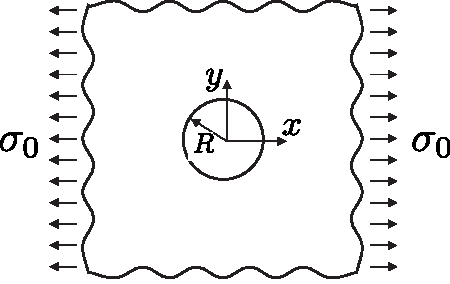
\includegraphics[width=0.4\textwidth]{figs/infinite-plate.pdf}	
	\caption{Infinite plate with a hole.}
	\label{Figure-4}
\end{figure}

The stress concentration predicted by Equations \eqref{eq:infiniteSX_XX}-\eqref{eq:infiniteSY_YY} decays
rather quickly away from the hole. Therefore, this solution can
be used for non-infinite plates, provided that the edges of the
plate are sufficiently far from the hole that the stresses on the
edges are approximately equal to the remote stress field. If this
is not the case, alternative solutions may
be used.

\subsection{Howland}

Howland\footnote{Howland, R.C.J.\ (1930). On the stresses in the
	neighbourhood of a circular hole in a strip under tension.
	Philosophical Transactions of the Royal Society of London A, 229,
	49-86.} derived semi-analytical expressions for the stress
concentration factors at the edge of a symmetric hole of radius
$R$ in a plate of finite width $2W$. These factors have been
calculated for a range of plate geometries and are shown in the
table below.

\vspace{10px}

\hspace{1cm} \begin{minipage}[]{8cm}
	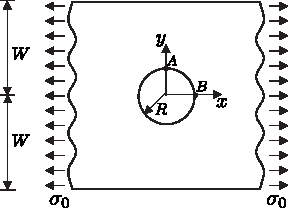
\includegraphics[width=0.8\textwidth]{figs/finite-plate.pdf} 
	\label{Figure-5}
\end{minipage} \hspace{1cm}
\begin{minipage}[]{6cm} Stress concentration factors\vspace{2mm}
	
	\begin{tabular}{c c c }
		\hline \hline
		$R/W$ & Point A & Point B \\
		& $\sigma_{xx}/\sigma_0$ & $\sigma_{yy}/\sigma_0$\\ \hline
		0 & 3.00 & -1.00 \\
		0.1 & 3.03 & -1.03 \\
		0.2 & 3.14 & -1.11 \\
		0.3 & 3.36 & -1.26 \\
		0.4 & 3.74 & -1.44 \\
		0.5 & 4.32 & -1.58 \\ \hline
	\end{tabular}
\end{minipage}

\centerline{Figure 5: Plate of finite width.}


\end{document}